% =====================================================================
% Electrical and Electronic Examples
% ---------------------------------------------------------------------
% Examples for the electrical and electronic engineering packages loaded
% in Base Packages.tex: circuitikz (symbol styles, op-amps, logic gates),
% tikz-timing, karnaugh-map, bodeplot, steinmetz, pgfplots 3D plots,
% bytefield, pdfpages and acronym. Delete whatever you do not need.
% =====================================================================

\section{Electrical and Electronic Examples}
\label{sec:electrical}

\subsection{Acronyms}

Acronyms are defined once in \texttt{Sections/Acronyms.tex} and written
with \verb|\ac{KEY}|. The first use is spelt out in full and later uses are
abbreviated: a \ac{MCU} generates a \ac{PWM} signal, and the \ac{MCU} also
reads an \ac{ADC}. Use \verb|\acp{KEY}| for plurals, e.g.\ two \acp{DAC}.
Only the acronyms you use appear in the list at the start of the report.

\subsection{Circuit Symbol Styles}

\texttt{circuitikz} can draw American (ANSI) or European (IEC) symbols.
Australian Standards (AS/NZS 1102) follow IEC symbols. Choose the style for
one diagram with \verb|\begin{circuitikz}[european]| or
\verb|[american]|, or for the whole report by adding the \verb|european|
option where \texttt{circuitikz} is loaded in \texttt{Base Packages.tex}.
\Cref{fig:divider} uses European symbols, while \cref{fig:rc-filter} uses
American symbols.

\Cref{fig:opamp} shows an op-amp, placed as a node and connected through
its \verb|.-|, \verb|.+| and \verb|.out| anchors. Its gain is given by
\cref{eq:opamp-gain}.
\begin{equation}
    V_\text{out} = -\frac{R_f}{R_\text{in}} V_\text{in}
    \label{eq:opamp-gain}
\end{equation}

\begin{figure}[H]
    \centering
    \begin{subfigure}[b]{0.45\linewidth}
        \centering
        \begin{circuitikz}[european]
            \draw (0,0) to[V, l=$V_\text{s}$] (0,4)
                        -- (2,4)
                        to[R, l=$R_1$] (2,2)
                        to[R, l=$R_2$] (2,0)
                        -- (0,0);
            \draw (2,2) to[short, *-o] (4,2) node[right] {$V_\text{out}$};
            \draw (2,0) to[short, *-o] (4,0);
        \end{circuitikz}
        \caption{}
        \label{fig:divider}
    \end{subfigure}
    \hfill
    \begin{subfigure}[b]{0.5\linewidth}
        \centering
        \begin{circuitikz}
            \draw (0,0) node[op amp] (opamp) {};
            \draw (opamp.-) to[R, l=$R_\text{in}$, -o] ++(-2.5,0) node[left] {$V_\text{in}$};
            \draw (opamp.-) -- ++(0,1.5) coordinate (top)
                  to[R, l=$R_f$] (top -| opamp.out) -- (opamp.out);
            \draw (opamp.out) to[short, *-o] ++(1,0) node[right] {$V_\text{out}$};
            \draw (opamp.+) -- ++(0,-0.5) node[ground] {};
        \end{circuitikz}
        \caption{}
        \label{fig:opamp}
    \end{subfigure}
    \caption{Further \texttt{circuitikz} examples. (a) Voltage divider (European symbols). (b) Inverting amplifier.}
    \label{fig:circuits}
\end{figure}

Logic gates are also nodes: \verb|european and port|,
\verb|european xor port| and so on (replace \verb|european| with
\verb|american| for the curved shapes). Inputs are the \verb|.in 1| and
\verb|.in 2| anchors and the output is \verb|.out|. \Cref{fig:half-adder}
is a half adder. Wires that cross without a dot are not connected.

\begin{figure}[H]
    \centering
    \begin{circuitikz}
        \draw (0,1.2) node[european xor port] (xor) {}
              (0,-1.2) node[european and port] (and) {};
        % Inputs
        \draw (xor.in 1) -- ++(-2.5,0) node[left] {$A$};
        \draw (xor.in 2) -- ++(-2.5,0) node[left] {$B$};
        \draw (and.in 1) -- ++(-1,0) coordinate (j1);
        \draw (j1) -- (j1 |- xor.in 1) node[circ] {};
        \draw (and.in 2) -- ++(-1.5,0) coordinate (j2);
        \draw (j2) -- (j2 |- xor.in 2) node[circ] {};
        % Outputs
        \draw (xor.out) -- ++(1,0) node[right] {$S$ (sum)};
        \draw (and.out) -- ++(1,0) node[right] {$C$ (carry)};
    \end{circuitikz}
    \caption{Half adder drawn with IEC logic gates.}
    \label{fig:half-adder}
\end{figure}

\subsection{Timing Diagrams}

\texttt{tikz-timing} draws digital signals from short letter codes:
\verb|L| low, \verb|H| high, \verb|Z| high impedance, \verb|C| clock
edge and \verb|D{text}| a data value. A number in front sets the width, so
\verb|2L| is low for two units and \verb|16{C}| is 16 clock edges. Every
row should add up to the same total width (20 units in
\cref{fig:spi-timing}, which shows one byte sent over \ac{SPI}).

\begin{figure}[H]
    \centering
    \begin{tikztimingtable}[timing/slope=0.2, xscale=2.5, yscale=1.5]
        SCLK                   & 2L 16{C} 2L \\
        $\overline{\text{CS}}$ & 1H 18L 1H \\
        MOSI                   & 2Z 2D{1} 2D{0} 2D{1} 2D{1} 2D{0} 2D{0} 2D{1} 2D{0} 2Z \\
        MISO                   & 2Z 16D{0x3C} 2Z \\
    \end{tikztimingtable}
    \caption{\acs{SPI} transfer of the byte \texttt{0xB2}.}
    \label{fig:spi-timing}
\end{figure}

Short signals can also be drawn in a sentence with
\verb|\texttiming{LHLHHL}|, which gives \texttiming{LHLHHL}.

\subsection{Karnaugh Maps}

The \texttt{karnaugh-map} environment takes the map size and variable
names. \verb|\minterms{...}| places the 1s, \verb|\autoterms[0]| fills
the remaining cells with 0s and \verb|\implicant{first}{last}| draws a
group from the first to the last cell. Groups that wrap around the edges
use \verb|\implicantedge| or \verb|\implicantcorner|.
\Cref{fig:kmap} simplifies to \cref{eq:kmap}.
\begin{equation}
    F = \overline{B}\,\overline{D} + BD
    \label{eq:kmap}
\end{equation}

\begin{figure}[H]
    \centering
    \begin{karnaugh-map}[4][4][1][$D$][$C$][$B$][$A$]
        \minterms{0,2,5,7,8,10,13,15}
        \autoterms[0]
        \implicant{5}{15}
        \implicantcorner
    \end{karnaugh-map}
    \caption{Karnaugh map of $F(A,B,C,D) = \sum m(0,2,5,7,8,10,13,15)$.}
    \label{fig:kmap}
\end{figure}

\subsection{Bode Plots from a Transfer Function}

\texttt{bodeplot} draws the magnitude and phase plots straight from the
poles, zeros and gain, so there is no need to work out the formula as in
\cref{fig:bode}. \Cref{fig:bodeplot} plots \cref{eq:tf}. Each pole at
$s = -a$ is entered as \verb|-a| in the \verb|p/{...}| list, zeros go in
\verb|z/{...}| and the gain in \verb|k/...|. The last two arguments are
the frequency range in \unit{\radian\per\second}.
\begin{equation}
    G(s) = \frac{10000}{(s + 10)(s + 1000)}
    \label{eq:tf}
\end{equation}

\begin{figure}[H]
    \centering
    \BodeZPK[plot/mag/{thick, blue}, plot/ph/{thick, blue}]
        {z/{}, p/{-10, -1000}, k/10000}{1}{1e5}
    \caption{Bode plot of $G(s)$ drawn with \texttt{bodeplot}.}
    \label{fig:bodeplot}
\end{figure}

\subsection{Phasors}

\texttt{steinmetz} provides \verb|\phase{angle}| for phasor notation.
\Cref{eq:phasor} applies Ohm's law to an AC circuit.
\begin{equation}
    \mathbf{I} = \frac{\mathbf{V}}{\mathbf{Z}}
    = \frac{\qty{230}{\volt}\phase{0^\circ}}{\qty{10}{\ohm}\phase{36.87^\circ}}
    = \qty{23}{\ampere}\phase{-36.87^\circ}
    \label{eq:phasor}
\end{equation}

\subsection{3D Plots}

\texttt{pgfplots} also draws in 3D with \verb|\addplot3|, and
\verb|view={azimuth}{elevation}| sets the viewing angle in degrees.
\Cref{fig:3d-wire} shows the magnetic field around a straight wire
carrying current $I$. The field lines are circles and the field strength
falls with distance, $B = \mu_0 I / (2\pi r)$, so the \verb|quiver| arrows
are scaled by $1/r$. The circles are repeated at several heights with
\verb|\pgfplotsforeachungrouped|.

\Cref{fig:3d-dipole} is a parametric surface: the radiation pattern of a
short dipole antenna, whose radiated power is proportional to
$\sin^2\theta$. Each point is given in spherical coordinates, with the
domain variables \verb|x| and \verb|y| used as $\theta$ and $\phi$, and
\verb|point meta| colours the surface by the radiated power. Note that
inside \verb|quiver| and \verb|point meta|, \verb|x|, \verb|y| and
\verb|z| are the coordinates of the plotted point, not the domain
variables.

\begin{figure}[H]
    \centering
    \begin{subfigure}[b]{0.49\linewidth}
        \centering
        \begin{tikzpicture}
            \begin{axis}[
                width=\linewidth,
                view={30}{25},
                hide axis, % Only the field and wire are shown
                xmin=-2, xmax=2, ymin=-2, ymax=2, zmin=-1.6, zmax=2,
            ]
                % Field lines and arrows at each height and radius
                \pgfplotsforeachungrouped \Z in {-1, 0, 1} {
                    \pgfplotsforeachungrouped \R in {0.7, 1.4} {
                        \addplot3[blue!60, domain=0:360, samples=50, samples y=0]
                            ({\R*cos(x)}, {\R*sin(x)}, \Z);
                        \addplot3[
                            blue, -Stealth, thick,
                            % Inside quiver, x and y are the point's coordinates
                            quiver={u={-0.4*y/(x^2+y^2)}, v={0.4*x/(x^2+y^2)}, w=0},
                            domain=0:270, samples=4, samples y=0,
                        ] ({\R*cos(x)}, {\R*sin(x)}, \Z);
                    }
                }
                % Current-carrying wire along the z-axis
                \addplot3[red, ultra thick, -Stealth] coordinates {(0,0,-1.6) (0,0,1.9)};
                \node[red, right] at (axis cs:0,0,1.8) {$I$};
                \node[blue, right] at (axis cs:1.4,0,1) {$\mathbf{B}$};
            \end{axis}
        \end{tikzpicture}
        \caption{}
        \label{fig:3d-wire}
    \end{subfigure}
    \hfill
    \begin{subfigure}[b]{0.49\linewidth}
        \centering
        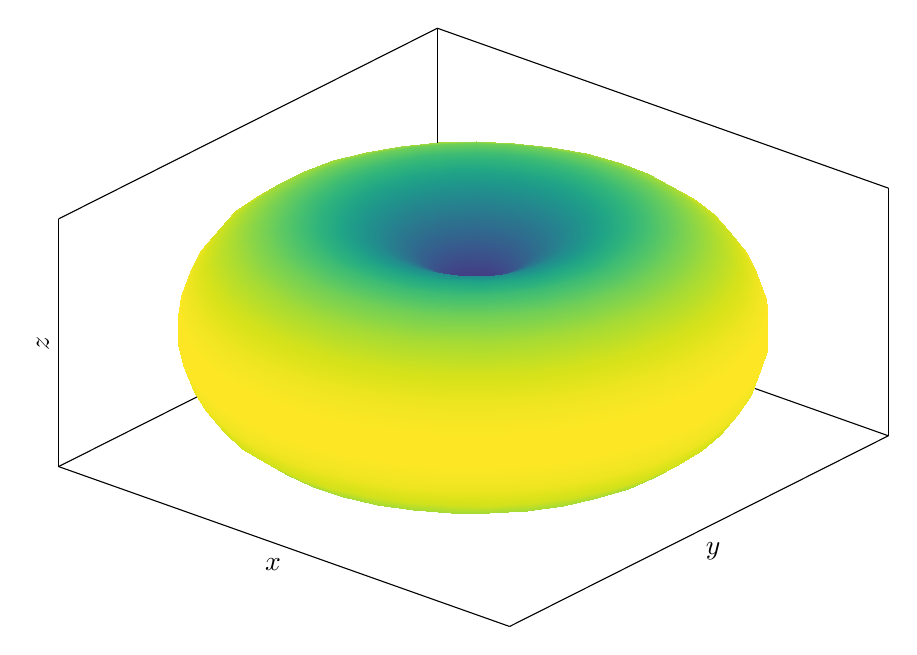
\begin{tikzpicture}
            \begin{axis}[
                width=\linewidth,
                view={40}{25},
                axis equal image,
                xlabel={$x$}, ylabel={$y$}, zlabel={$z$},
                ticks=none,
                colormap/viridis,
            ]
                \addplot3[
                    surf, shader=interp, z buffer=sort,
                    domain=0:180, y domain=0:360,
                    samples=30, samples y=40,
                    % Colour by distance from the origin (the radiated power)
                    point meta={sqrt(x^2+y^2+z^2)},
                ] ({sin(x)^3*cos(y)}, {sin(x)^3*sin(y)}, {sin(x)^2*cos(x)});
            \end{axis}
        \end{tikzpicture}
        \caption{}
        \label{fig:3d-dipole}
    \end{subfigure}
    \caption{3D plots drawn with \texttt{pgfplots}. (a) Magnetic field around a straight wire. (b) Radiation pattern of a short dipole.}
    \label{fig:3d}
\end{figure}

\subsection{Registers and Data Frames}

\texttt{bytefield} draws register maps and communication frames. Each
\verb|\bitbox{width}{text}| is one field, \verb|width| bits wide, and
\verb|\bitheader{0-7}| numbers the bits. \Cref{fig:register} is an 8-bit
control register and \cref{fig:uart-frame} is a \ac{UART} frame.

\begin{figure}[H]
    \centering
    \begin{bytefield}[bitwidth=3.5em, endianness=big]{8}
        \bitheader{0-7} \\
        \bitbox{1}{EN} \bitbox{2}{MODE[1:0]} \bitbox{3}{PRESCALE[2:0]}
        \bitbox{1}{IE} \bitbox{1}{\color{gray}--}
    \end{bytefield}
    \caption{Timer control register. Bit 0 is reserved.}
    \label{fig:register}
\end{figure}

\begin{figure}[H]
    \centering
    \begin{bytefield}[bitwidth=3em]{11}
        \bitbox{1}{Start} \bitbox{1}{D0} \bitbox{1}{D1} \bitbox{1}{D2}
        \bitbox{1}{D3} \bitbox{1}{D4} \bitbox{1}{D5} \bitbox{1}{D6}
        \bitbox{1}{D7} \bitbox{1}{Parity} \bitbox{1}{Stop}
    \end{bytefield}
    \caption{\acs{UART} frame with 8 data bits (sent LSB first), even parity and one stop bit.}
    \label{fig:uart-frame}
\end{figure}

\subsection{Datasheets and External PDFs}

Whole pages from a PDF, such as a datasheet or a schematic exported from
KiCad or Altium, are added with \verb|\includepdf| from \texttt{pdfpages}.
Use \verb|pages=-| for every page or \verb|pages={1,3-5}| for a selection.
See \cref{app:datasheet} for an example.

\cleardoublepage
